\RequirePackage{fix-cm}
\documentclass{article}
\usepackage{graphicx}
\usepackage{xcolor}
\usepackage{background}
\usepackage{tikz}
\usepackage{float}
\usepackage{eso-pic}
\usepackage{hyperref}


% Imposta il background per la prima pagina
\backgroundsetup{
    scale=1,
    color=black,
    opacity=1,
    angle=0,
    contents={
        \begin{tikzpicture}[overlay, remember picture]
            \node[inner sep=0pt, anchor=center] at (current page.center) {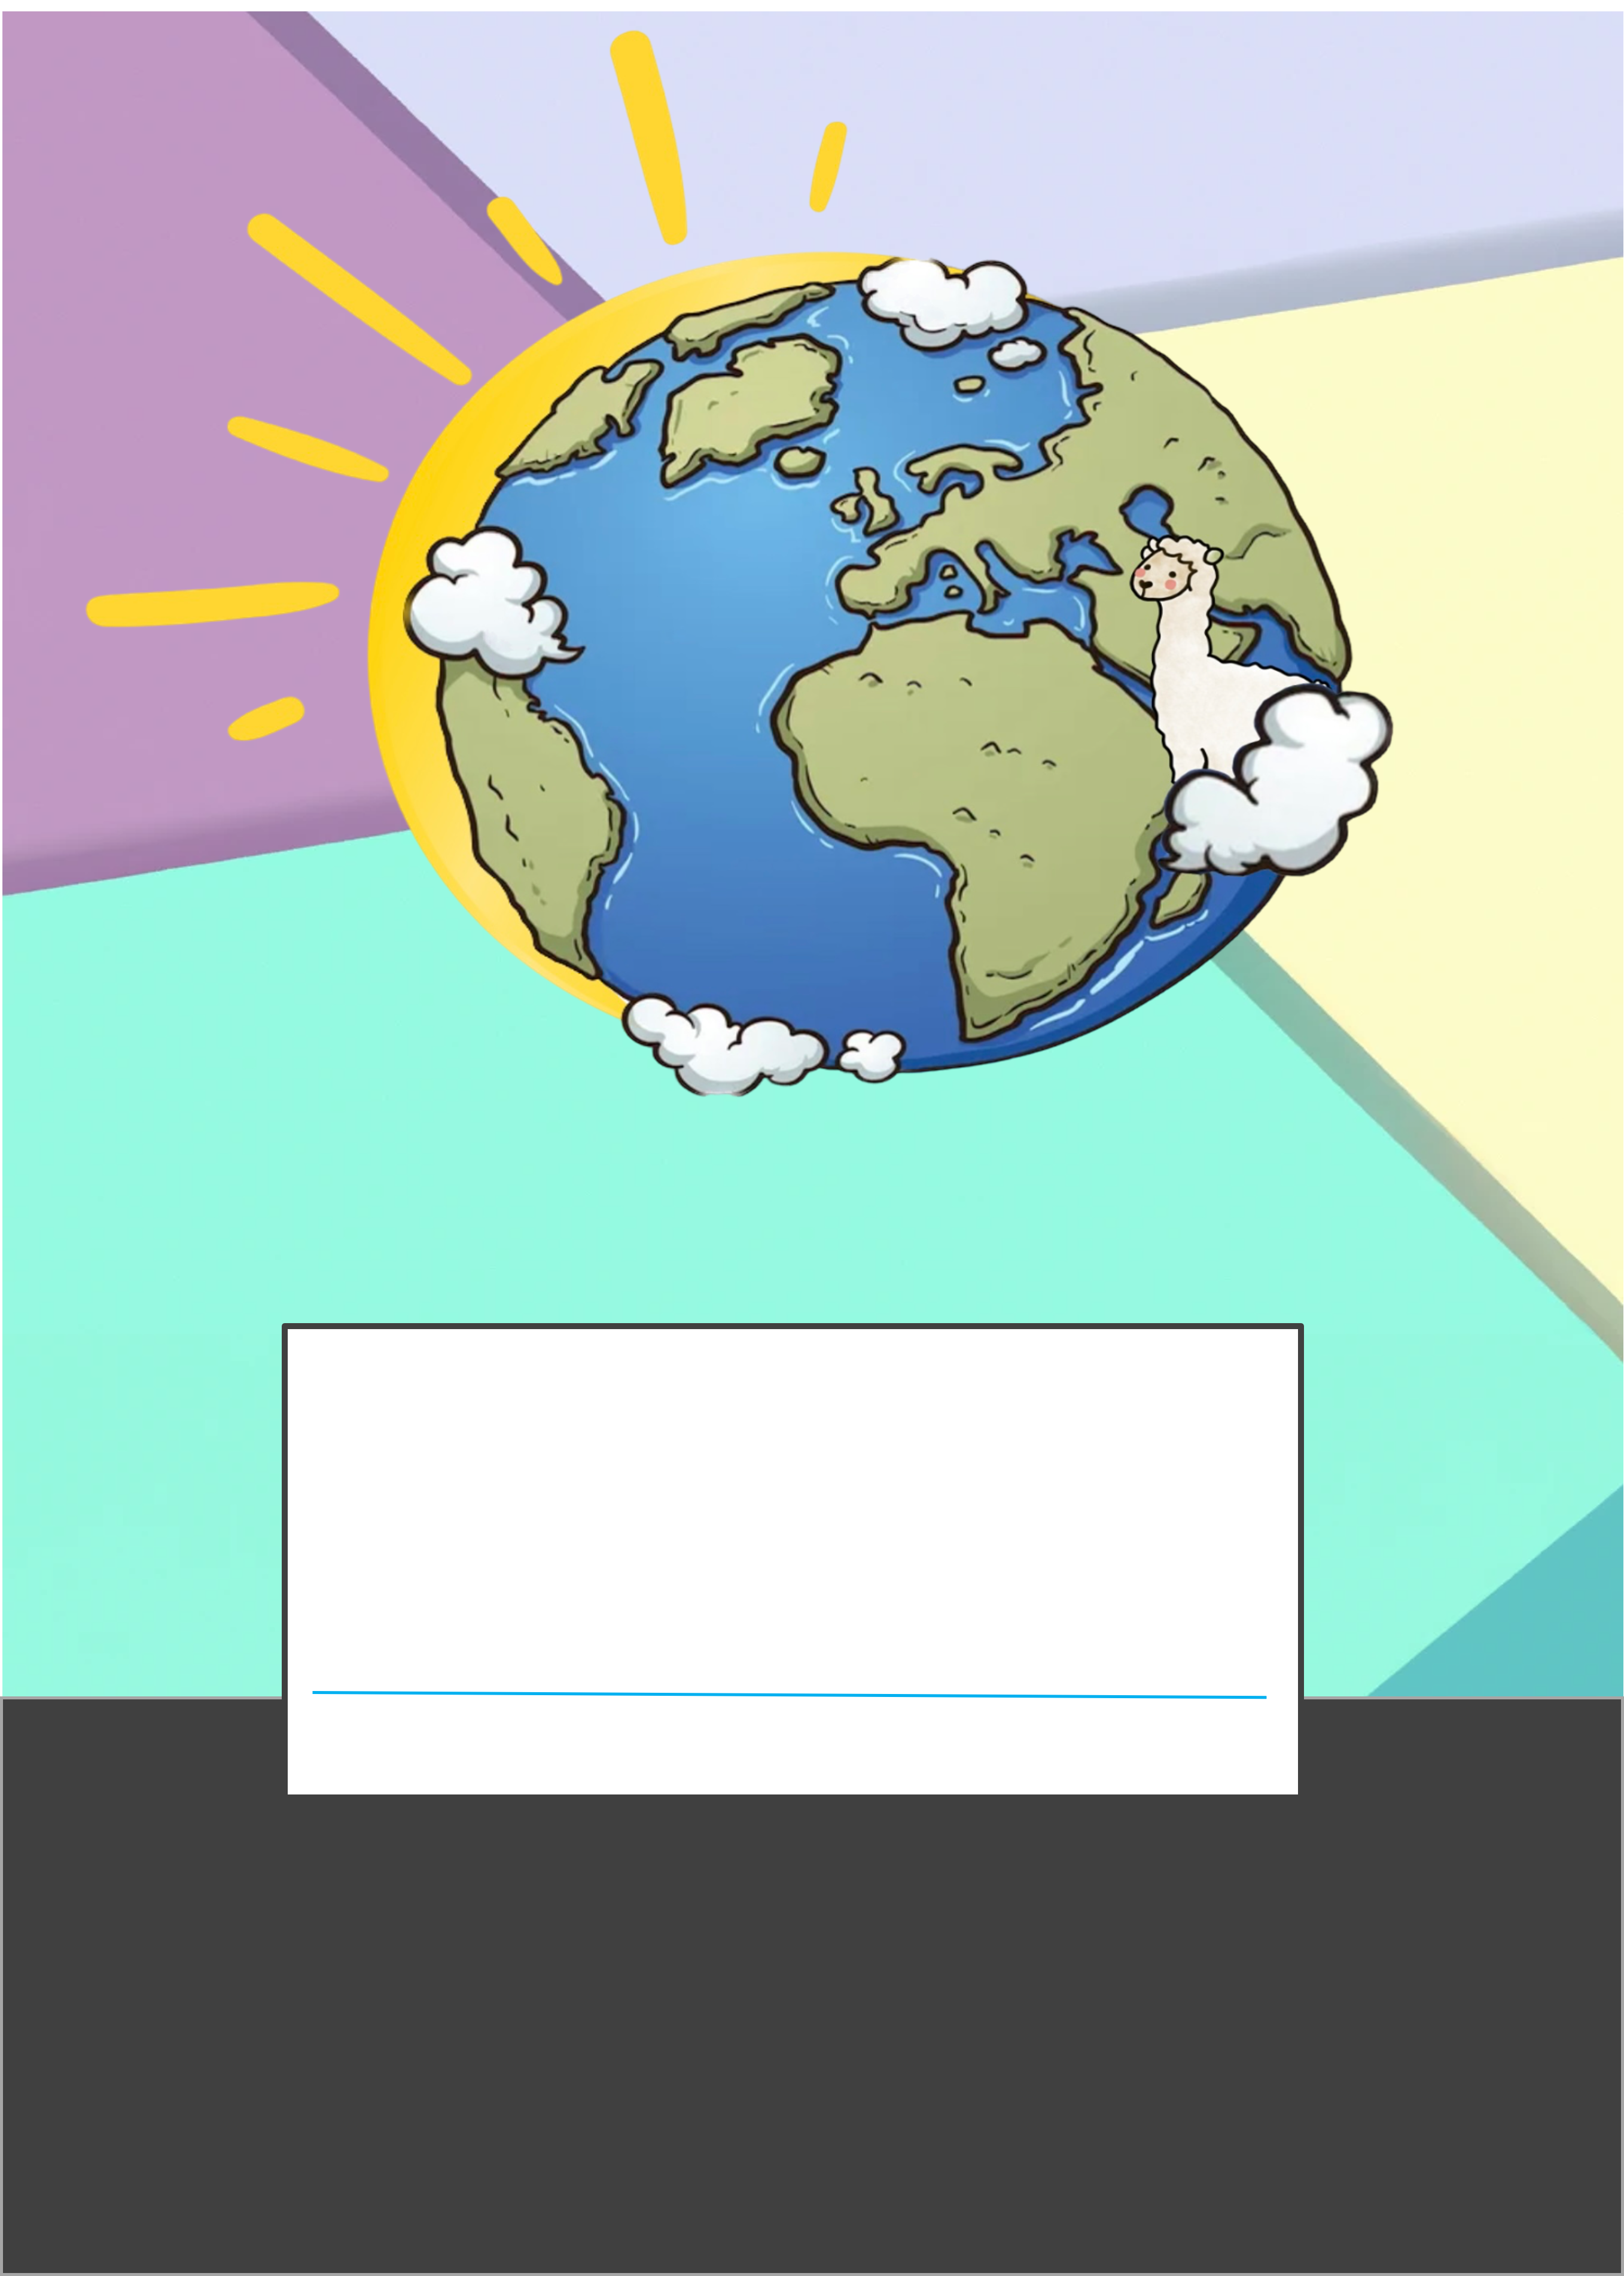
\includegraphics[width=\paperwidth,height=\paperheight,keepaspectratio]{../../img/firstpage_background.png}};
            \node[text=cyan, font=\fontsize{35}{50}\selectfont\bfseries] at ([xshift=-0.2cm,yshift=-4.5cm]current page.center) {Climate Monitoring};
            \node[text=cyan, font=\large] at ([xshift=-0.4cm,yshift=-7.5cm]current page.center) {\textit{Manuale Utente}};
            \node[text=white, font=\large] at ([xshift=-8.5cm,yshift=-9cm]current page.center) {Autori:};
            \node[text=white, font=\large] at ([xshift=-6.85cm,yshift=-10.5cm]current page.center) {Andrea Tettamanti 745387};
            \node[text=white, font=\large] at ([xshift=-7.28cm,yshift=-11.5cm]current page.center) {Luca Mascetti 752951};
            \node[text=white, font=\large] at ([xshift = 8cm, yshift = -9cm]current page.center) {Versione: 1.1};
            \node[text=white, font=\large] at ([xshift = 8cm, yshift = -10cm]current page.center) {Data: 07-02-2024};
        \end{tikzpicture}    }
}

\begin{document}

%frontespizio
\begin{titlepage}
    \null
\end{titlepage}

% Sovrapponi l'immagine al numero di pagina
\AddToShipoutPictureBG{
    \begin{tikzpicture}[overlay, remember picture]
        \node[inner sep=0pt, anchor=south] at ([xshift=-0.15cm,yshift=2.7cm]current page.south) {
\includegraphics[width=1.5cm,height=1.5cm]{../../img/number page.png}};
    \end{tikzpicture}
}

\clearpage
\NoBgThispage
\tableofcontents
\listoffigures
\clearpage

\NoBgThispage
\section{Introduzione}
Benvenuti nell'applicazione \emph{Climate Monitoring}, software progettato per fornire accesso ai dati climatici 
provenienti dai centri di monitoraggio in tutta Italia. Questa applicazione è stata sviluppata con l'obiettivo di 
mettere a disposizione degli operatori ambientali e dei cittadini comuni dati accurati e rilevanti relativi alle 
condizioni climatiche della propria zona di interesse.

\NoBgThispage
\section{Installazione}
\subsection{Requisiti Minimi}
Per eseguire l’applicazione è necessario una versione recente di \textbf{Java JDK}, non superiore alla \textbf{17}, e sistema 
operativo \textbf{Windows 10} e successivi (L’applicazione può essere eseguita anche su versioni precedenti di 
Windows e altri SO quali MAC e Linux, ma non è garantito l’esatto funzionamento).

\subsection{Installazione}
Scaricare la cartella ZIP denominata “Tettamanti\_745387” ed estrarla. All’interno della cartella 
estratta, fare click su “InstallClimateMonitoringApp”. Una volta che l’installazione è finita, apparirà
il collegamento dell’app sul desktop.\\
\textcolor{red}{ATTENZIONE}: se si tenta di installare l’applicazione o far partire il file .jar all’interno della cartella 
ZIP, questi non funzioneranno/daranno errore.
\NoBgThispage
\section{Esecuzione ed Uso}

\subsection{Avviare l'applicazione}
Per avviare l'applicazione assicurarsi di seguire questi passaggi:
\begin{itemize}
    \item Avere PostgreSQL in esecuzione;
    \item Aprire il terminale nella cartella\\ \texttt{$C:/Program Files/Tettamanti\_745387/JarFIle/artifacts/ClimateMonitoringJar$};
    \item Digitare il comando \texttt{java -jar Server.jar [host password]}. Il server deve sempre partire prima del client, in quanto il client si connette al server;
    \item Per far partire il client ci sono due opzioni:
    \begin{itemize}
        \item Aprire un nuovo terminale nella cartella\\ \texttt{$C:/Program Files/Tettamanti\_745387/JarFIle/artifacts/ClimateMonitoringJar$} e
        digitare il comando \texttt{java -jar Client.jar};
        \item Fare doppio click sul collegamento che si è creato sul desktop dopo l'installazione.
    \end{itemize}
\end{itemize}

\textcolor{red}{ATTENZIONE}: il server rimane attivo per 5 minuti. Se non riceve richieste dall'applicazione, si spegnerà automaticamente. Per riavviare il server, chiudere il terminale e ripetere i passaggi sopra descritti.



\subsection{Schermata Home}
Dopo una breve schermata di caricamento, verrà visualizzata la schermata Home:
\begin{figure}[H]
    \centering
    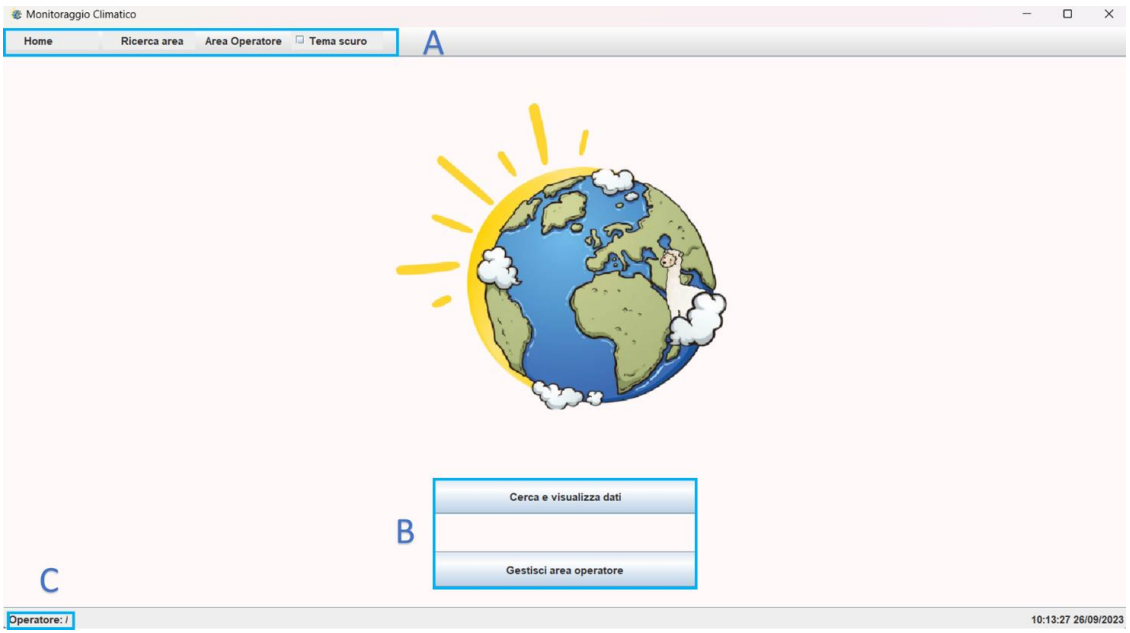
\includegraphics[width=1\textwidth]{../../img/schermata_home.png}
    \caption{Schermata Home}
\end{figure}

\begin{enumerate}
\renewcommand{\labelenumi}{\Alph{enumi}}
    \item \textbf{Barra del menu:} 
    \begin{itemize}
        \item \textbf{Home:} visualizza la schermata principale dell'applicazione senza modificare i dati di accesso dell'operatore corrente.
        \item \textbf{Ricerca area:} permette di accedere alla schermata adibita alla ricerca di un'area specifica.
        \item \textbf{Area Operatore:} permette di accedere alla schermata adibita alla registrazione e accesso per gli operatori.
        \item \textbf{Tema scuro:} permette di attivare o disattivare il tema scuro dell'applicazione.
    \end{itemize} 
    \item \textbf{Pulsanti principali:}
    \begin{itemize}
        \item \textbf{Cerca e visualizza dati:} ha la stessa funzione di \emph{Ricerca area} nella barra del menu.
        \item \textbf{Gestici area operatore:} ha la stessa funzione di \emph{Area Operatore} nella barra del menu.
    \end{itemize}
    \item \textbf{Operaore:} visualizza il nome dell'operatore corrente; se non è stato effettuato l'accesso, verrà visualizzato il carattere /.
\end{enumerate}
\subsection{Ricerca area}
Dopo aver cliccato il pulsante \emph{Cerca e visualizza dati} nella schermata Home, verrà visualizzata la schermata di ricerca area:
\begin{figure}[H]
    \centering
    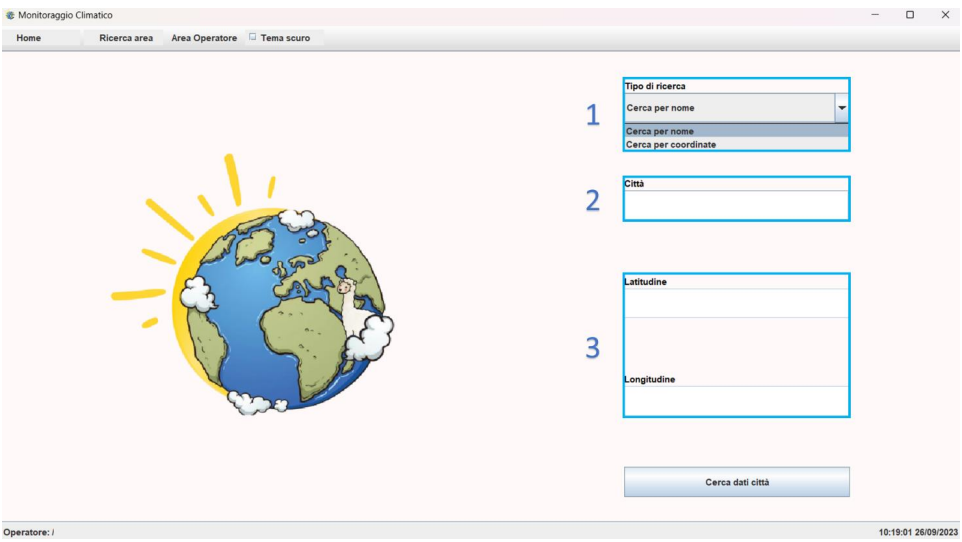
\includegraphics[width=1\textwidth]{../../img/schermata_ricerca_area.png}
    \caption{Schermata Ricerca area}
\end{figure}
Qui è possibile selezionare che tipo di ricerca [1] si vuole effetuare:
\begin{itemize}
    \item \textbf{Ricerca per nome:} permette di cercare un'area speci
    fica inserendo il nome dell'area nell'apposito campo [2].
    \item \textbf{Ricerca per coordinate:} permette di cercare un'area specifica inserendo le coordinate geografiche negli appositi campi [3]
    (Es. 45,123456  9,123456).
\end{itemize}

Quando si clicca il pulsante \emph{Cerca dati città}, se nel sistema sono presenti più città con lo stesso nome o le coordinate insertie fanno riferimento
ad un'area che comprende più città, apparirà un avviso che consente di scegliere la città desiderata: 
\begin{figure}[H]
    \centering
    \includegraphics[width=1\textwidth]{../../img/scelta_città.png}
    \caption{Schermata di scelta della città}
\end{figure} 
\input{Dati città sub.tex}
\subsection{Area operatore}
Dopo aver cliccato il pulsante \emph{Gestisci area operatore} nella schermata Home, verrà visualizzata la schermata di accesso e registrazione per gli operatori:
\begin{figure}[H]
    \centering
    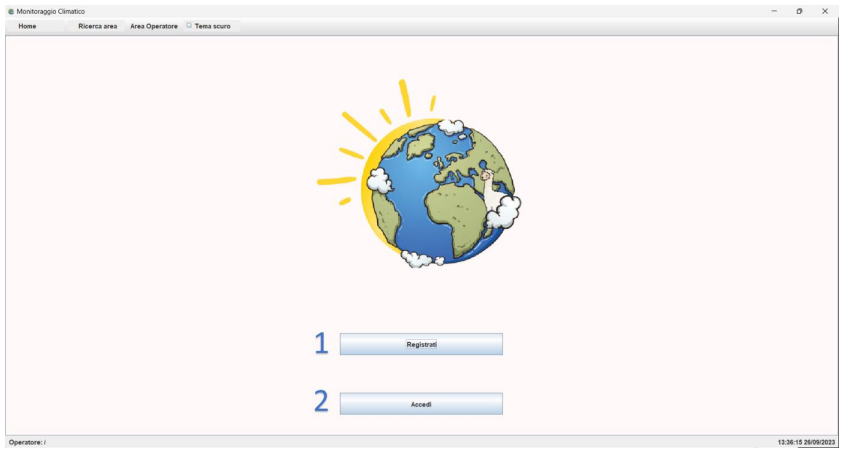
\includegraphics[width=1\textwidth]{../../img/schermata_area_operatore.png}
    \caption{Schermata Area operatore}
\end{figure}

Il pulsante \emph{Registrati} permette di accedere alla schermata di registrazione:
\begin{figure}[H]
    \centering
    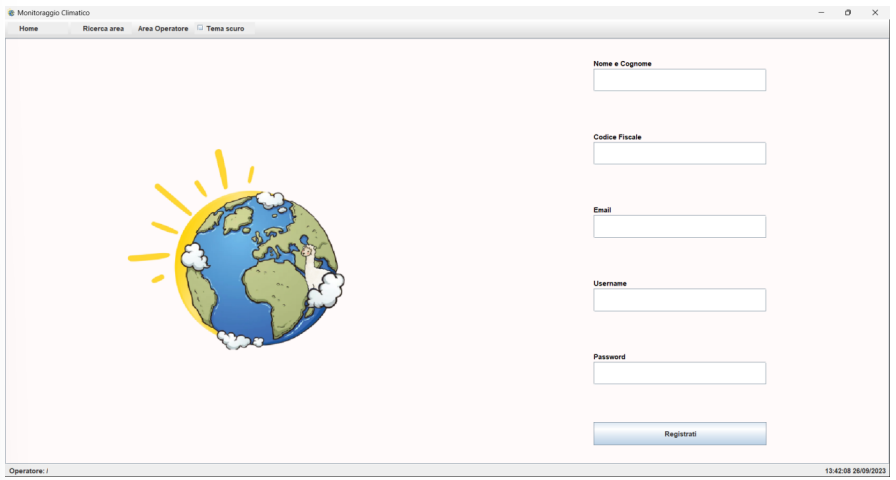
\includegraphics[width=1\textwidth]{../../img/schermata_registrazione.png}
    \caption{Schermata Registrazione}
\end{figure}

Qui è possibile inserire i propri dati personali e scegliere un nome utente e una password per accedere all'applicazione:
\begin{itemize}
    \item Nome e Cognome (Es. Mario Rossi).
    \item Codice fiscale (Es. RSSMRA01A01H501A).
    \item E-mail (Es. mario.rossi@gmail.com).
    \item Username (Es. MarioRossi).
    \item Password (Es. MarioRossi00!).
\end{itemize}

Una volta inseriti correttamente i dati, cliccare il pulsante \emph{Registrati} per completare la registrazione.

Dopo aver effettuato la registrazione, è possibile effettuare l'accesso inserendo il proprio username e la propria password nella schermata di accesso:
\begin{figure}[H]
    \centering
    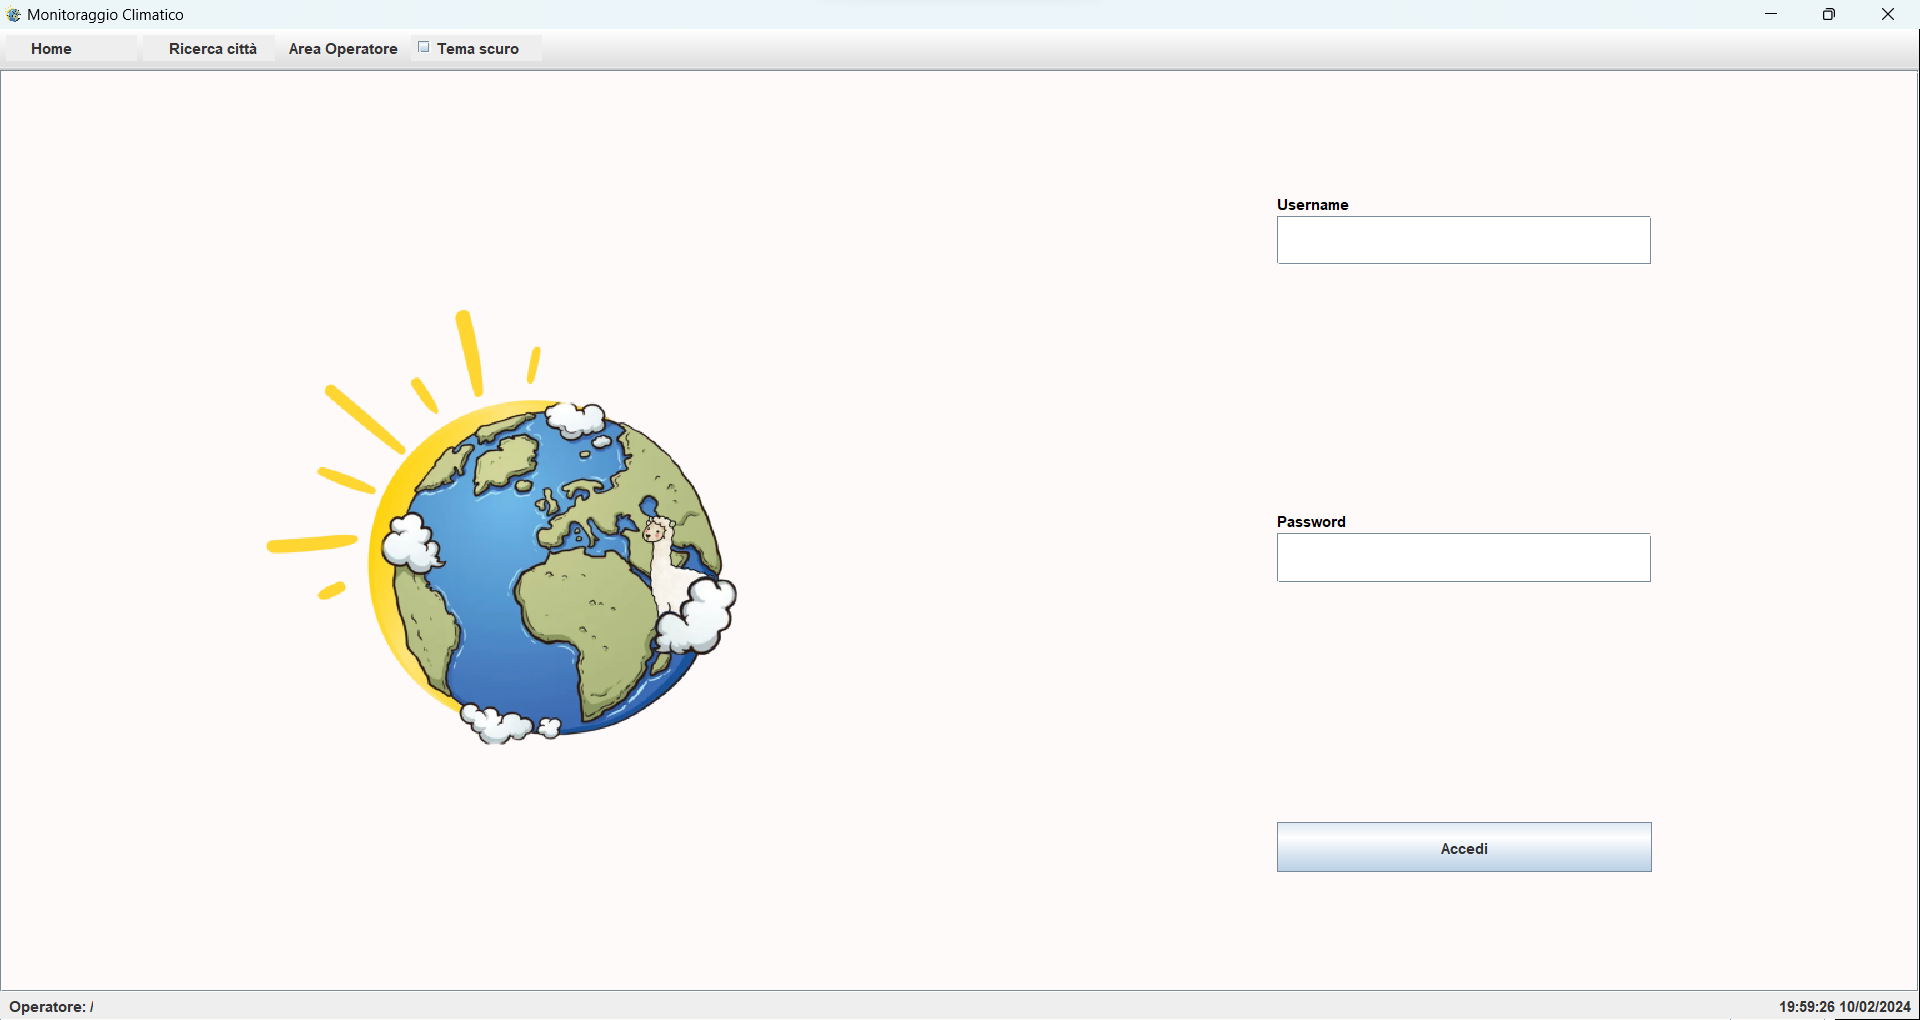
\includegraphics[width=1\textwidth]{../../img/schermata_login.png}
    \caption{Schermata Accesso}
\end{figure}

Una volta effettuato l'accesso, apparirà la seguente finestra: 
\begin{figure}[H]
    \centering
    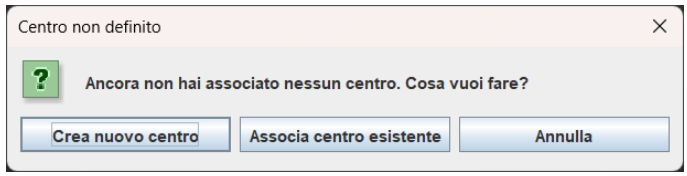
\includegraphics[width=1\textwidth]{../../img/finestra_centro.png}
    \caption{Finestra di dialogo Centro}
\end{figure}

Se si clicca \emph{Associa centro esistente} vengono viasualizzati, se presenti, i centri di monitoraggio nel sistema:
\begin{figure}[H]
    \centering
    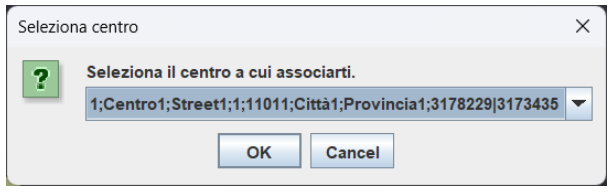
\includegraphics[width=1\textwidth]{../../img/seleziona_centro.png}
    \caption{Finestra di dialogo per la selezione del centro}
\end{figure}

Se il centro a cui ci si vuole associare non è presentare, cliccando \emph{Cancel} si torna alla finestra precedente e si può procedere a creare il prorpio
centro di monitoraggio inserendo i dati relativi ad esso:
\begin{figure}[H]
    \centering
    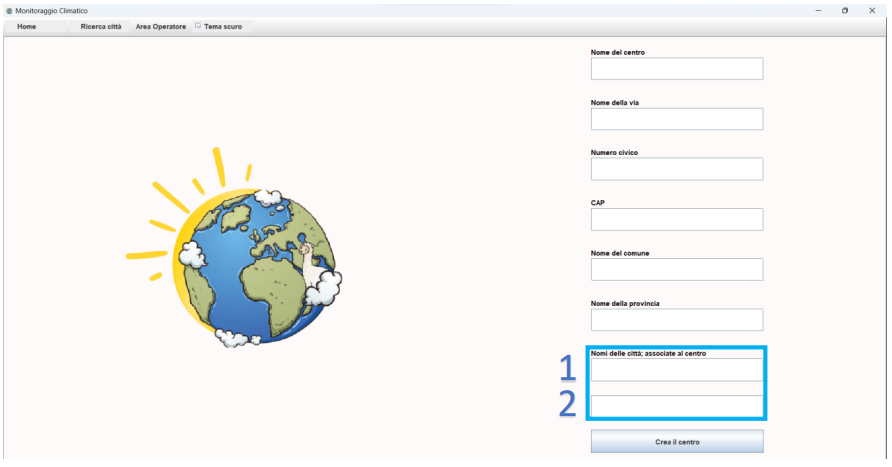
\includegraphics[width=1\textwidth]{../../img/schermata_creazione_centro.png}
    \caption{Schermata Creazione centro}
\end{figure}

Per inserire correttamente il nome delle città, si scrive il suo nome nel campo [1] e si preme il pulsante \emph{Invio}; se sono presenti più città
con lo stesso nome,
sarà possibile specificare quale aggiungere scegliendo dal menù che appare: 
\begin{figure}[H]
    \centering
    \includegraphics[width=1\textwidth]{../../img/scelta_città.png}
    \caption{Finestra per la scelta della città}
\end{figure}

Una volta selezionata la città desiderata, comparirà nel campo [2] con i sui dati geografici associati:
\begin{figure}[H]
    \centering
    \includegraphics[width=0.7\textwidth]{../../img/esempio_città_associata.png}
    \caption{Esempio città associata correttamente}
\end{figure}

Questo procedimento si ripete per ogni città che si vuole associare al centro di monitoraggio.\\
Se si sbaglia ad inserire una città, è possibile rimuoverla cliccando sul suo nome nel campo [2] ed eliminandola:
\begin{figure}[H]
    \centering
    \includegraphics[width=1\textwidth]{../../img/esempio_città_eliminata.png}
    \caption{Esempio città rimossa correttamente}
\end{figure}

\textcolor{red}{ATTENZIONE:} una volta creato un centro di monitoraggio, non è possibile modificare i dati inseriti o eliminarlo.\\
\subsection{Inserimento dati climatici per una città}
Ora che il centro di monitoraggio è stato creato, è possibile inserire i dati climatici per le città associate ad esso.\\ 

\begin{figure}[H]
    \centering
    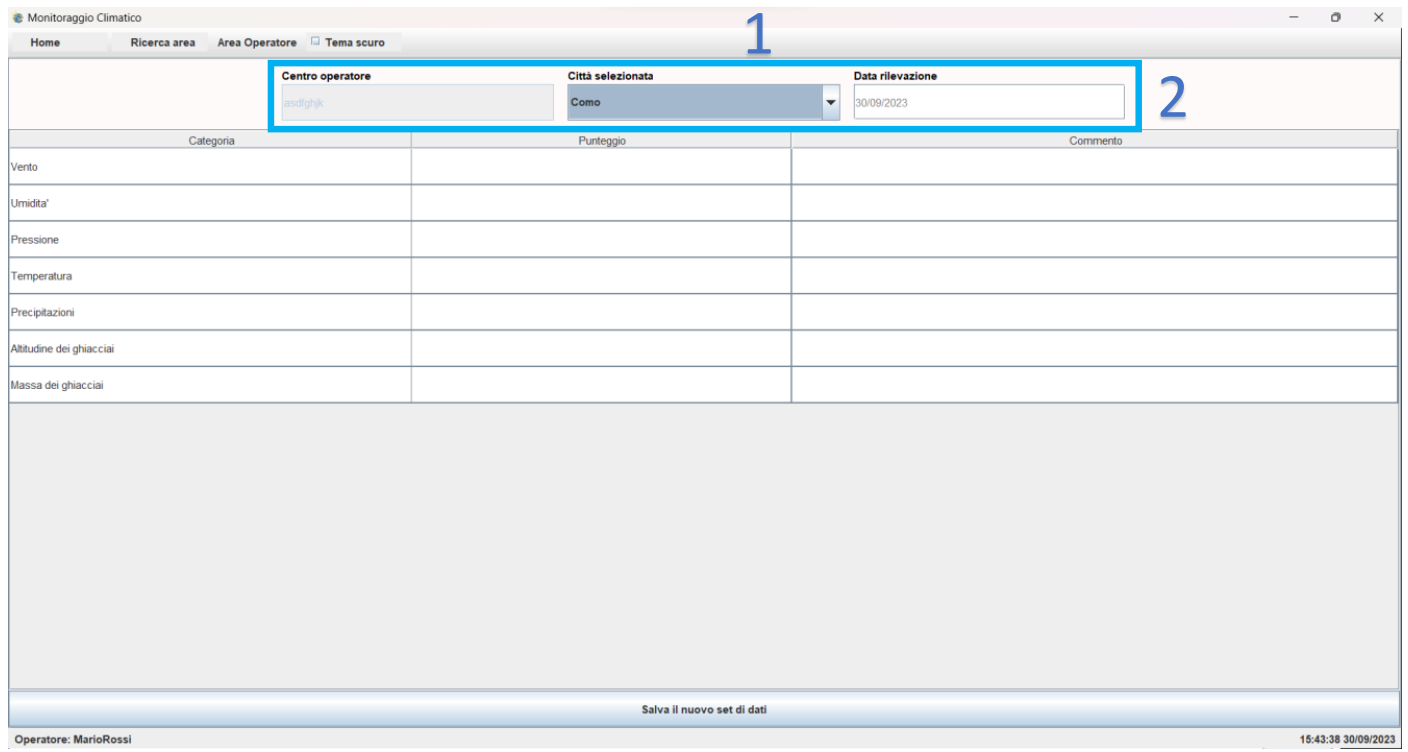
\includegraphics[width=1\textwidth]{../../img/schermata_inserimento_dati.png}
    \caption{Schermata Inserimento dati}
\end{figure}

Nel campo [1] è possibile scegliere per quale città si vogliono inserire i dati climatici, mentre nel campo [2] è possibile scegliere per quale data
si vogliono inserire i dati.
Se non viene modificata la data, verrà inserita la data corrente.\\

Nella tabella sottostante, nella colonna \emph{Punteggio} è possibile inserire il punteggio relativo al parametro climatico in un range da 1 a 5.
Per sapere la suddivisione in fasce dei punteggi, fare riferimento alla sezione \ref{sec:legenda_punteggi} del presente manuale
oppure cliccare sulla categoria desiderata per visualizzare la relativa legenda.\\

\begin{figure}[H]
    \centering
    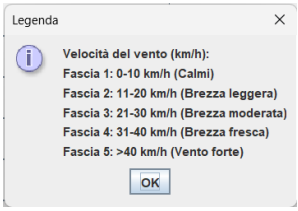
\includegraphics[width=0.7\textwidth]{../../img/esempio_legenda.png}
    \caption{Esempio di legenda}
\end{figure}

Per poter salvare i dati nel sistema, bisogna obbligatoriamente inserire almeno un punteggio. Inoltre, nella colonna \emph{Commento} è possibile
inserire un commento relativo al punteggio inserito, con un limite di 256 caratteri.
Se vengono superati, verrà visualizzato un messaggio di errore e non si potranno salvare i dati a meno che i commenti non rispettino il limite.

\begin{figure}[H]
    \centering
    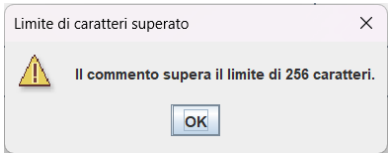
\includegraphics[width=0.7\textwidth]{../../img/avviso_limite_caratteri.png}
    \caption{Avviso limite caratteri}
\end{figure}

Per salvare correttamente i dati premere \emph{Invio} prima di cliccare il pulsante \emph{Salva il nuovo set di dati}.
Una volta salvati i dati, questi potranno essere visuallizati in \ref{sec:dati_città}.\\
\subsection{Tema scuro}
Per attivare o disattivare il tema scuro dell'applicazione, cliccare il pulsante \emph{Tema scuro} nella barra del menu:
\begin{figure}[H]
    \centering
    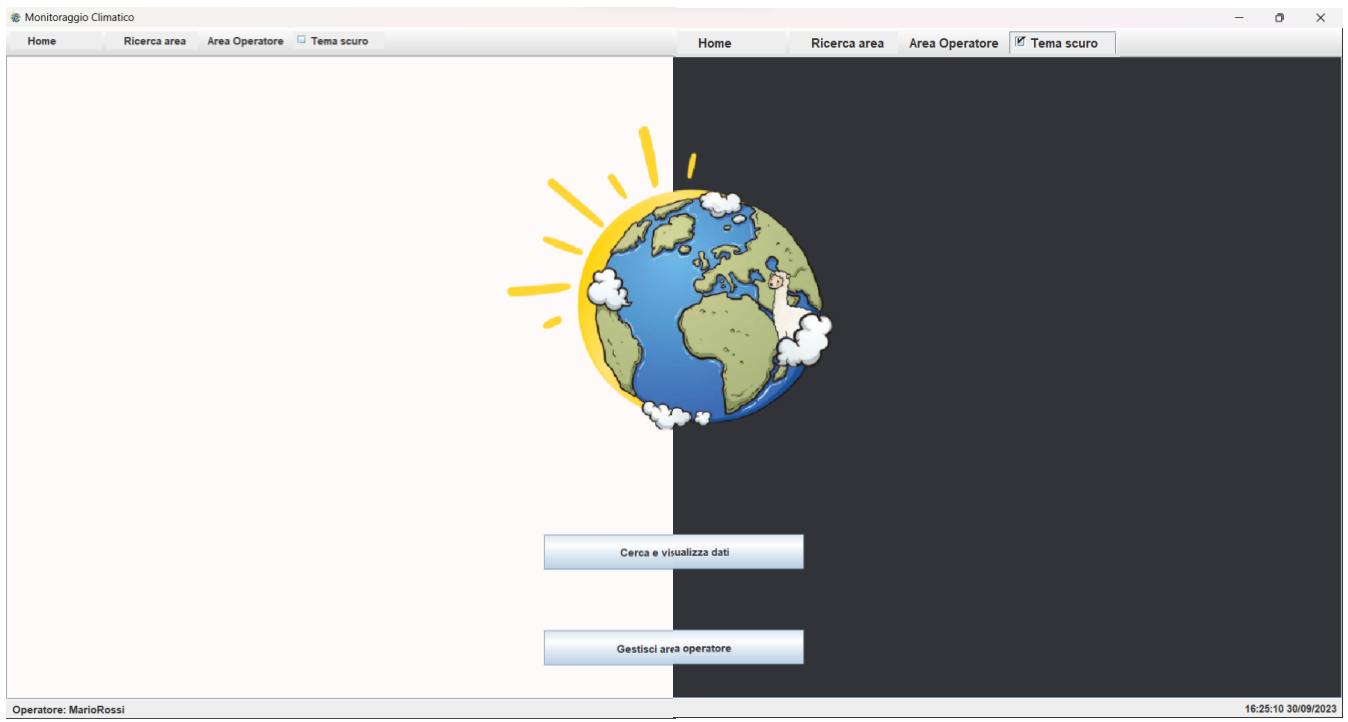
\includegraphics[width=1\textwidth]{../../img/tema_scuro.png}
    \caption{Attivazione e disattivazione del tema scuro}
\end{figure}
\section{Uscire dall'applicazione}
Per uscire dall'applicazione, cliccare il pulsante \emph{X} in alto a destra della finestra dell'applicazione.
\section {Legenda punteggi}
\label{sec:legenda_punteggi}
\begin{figure}[H]
    \centering
    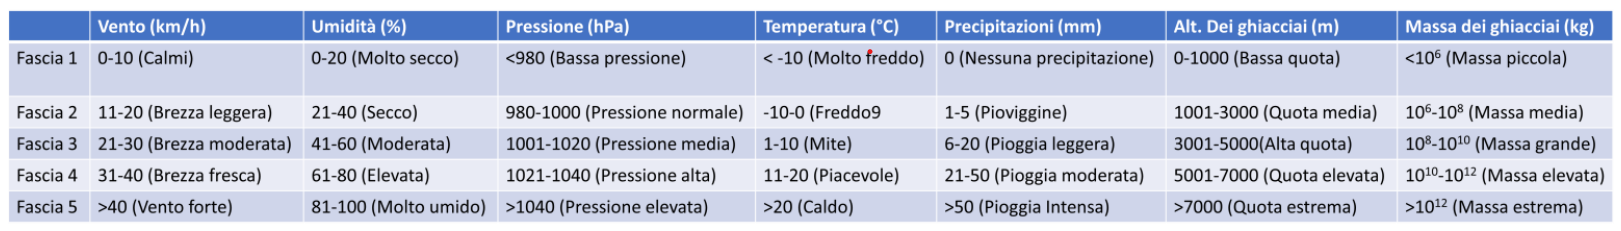
\includegraphics[width=1.2\textwidth]{../../img/legenda_punteggi.png}
    \caption{Legenda punteggi}
\end{figure}

\end{document}
